\documentclass{article}

\usepackage{tikz}
\usetikzlibrary{calc, automata, chains, arrows.meta}


\begin{document}

\begin{figure}
    \centering
    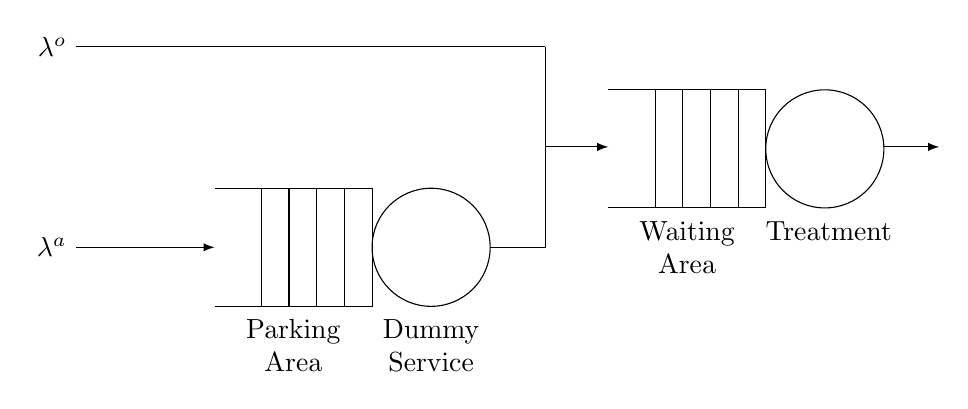
\begin{tikzpicture}[>=latex]
        % the rectangle with vertical rules (Queue 1)
        \draw (0,0) -- ++(2cm,0) -- ++(0,-1.5cm) -- ++(-2cm,0);
        \foreach \i in {1,...,4}
        \draw (2cm-\i*10pt,0) -- +(0,-1.5cm);
        
        % the circle (Queue 1)
        \draw (2.75,-0.75cm) circle [radius=0.75cm];

        % the rectangle with vertical rules (Queue 2)
        \draw (5,1.25) -- ++(2cm,0) -- ++(0,-1.5cm) -- ++(-2cm,0);
        \foreach \i in {1,...,4}
        \draw (7cm-\i*10pt,1.25) -- +(0,-1.5cm);

        % the circle (Queue 2)
        \draw (7.75,0.5) circle [radius=0.75cm];

        % the arrows and labels (Queue 1+2)
        \draw[-] (3.5,-0.75) -- +(20pt,0);
        \draw[<-] (0,-0.75) -- +(-50pt,0) node[left] {$\lambda^a$};
        \draw[->] (8.5,0.525) -- +(20pt,0);
        \node[align=center] at (1cm,-2cm) {Parking \\ Area};
        \node[align=center] at (2.75cm,-2cm) {Dummy \\ Service};
        \node[align=center] at (6cm,-0.75cm) {Waiting \\ Area};
        \node[align=center] at (7.8cm,-0.75cm) {Treatment \\ };
        
        \draw (4.2, 1.8) -- +(-169.5pt,0) node[left] {$\lambda^o$};
        \draw (4.2, 1.8) -- (4.2, -0.75);
        \draw[->] (4.2, 0.525) -- (5, 0.525);

    \end{tikzpicture}

\end{figure}

\end{document}